% Created 2013-10-12 sob 10:39
\documentclass[presentation,aspectratio=43,12pt]{beamer}
\usepackage{fontspec}
\usepackage{fixltx2e}
\usepackage{graphicx}
\usepackage{longtable}
\usepackage{float}
\usepackage{wrapfig}
\usepackage{soul}
\usepackage{textcomp}
\usepackage{marvosym}
\usepackage{wasysym}
\usepackage{latexsym}
\usepackage{amssymb}
\usepackage{amstext}
\usepackage{hyperref}
\tolerance=1000
\usepackage{pgfpages}
\usepackage{tikz}
\institute[SRPOL]{Samsung R\&D Institute Poland}
\renewcommand\pgfsetupphysicalpagesizes{\pdfpagewidth\pgfphysicalwidth\pdfpageheight\pgfphysicalheight}
\AtBeginSection[]{{\setbeamertemplate{footline}{}\setbeamertemplate{background canvas}[section page]\begin{frame}<beamer>\sectionpage\end{frame}\setbeamertemplate{footline}[tizen]}}
\hypersetup{colorlinks=true,linkcolor=,urlcolor=pantone326}
\usetheme{jesien}
\author{Karol Lewandowski}
\date{11–13 Październik, 2013}
\title{Tizen, czyli trudna droga od systemu wbudowanego do nowoczesnego GNU/Linuksa}
\hypersetup{
  pdfkeywords={},
  pdfsubject={},
  pdfcreator={Emacs 23.3.1 (Org mode 8.0.7)}}
\begin{document}

\maketitle
\begin{frame}{Outline}
\tableofcontents
\end{frame}



\section{Wstęp}
\label{sec-1}

\begin{frame}[label=sec-1-1]{Wprowadzenie}
Celem prezentacji jest przybliżenie procesów, problemów i~ich
rozwiązań związanych z budową solidnej bazy systemu operacyjnego,
czyli dystrybucji GNU/Linuksa.

\note{Płytki uruchomieniowe i deweloperskie (ale nie produkty):

\begin{itemize}
\item RD-PQ Odroid, Origen, Armdale
\end{itemize}

Kernelu - temat na \emph{cykl} prezentacji

\begin{itemize}
\item Wsparcie dla platformy Samsung Exynos (sterowniki SoC)
\item DMA-BUF
\item Video4Linux2 Multiplane
\item Contigous Memory Allocator (CMA)
\end{itemize}}
\end{frame}

\begin{frame}[label=sec-1-2]{Tizen: Dystrybucja GNU/Linuksa}
\begin{itemize}
\item Dystrybucja GNU/Linuksa ze standardowymi komponentami:
\begin{itemize}
\item Jądro Linux
\item Narzędzia GNU
\item Xorg
\end{itemize}

\item \ldots{} jak również trochę mniej standardowymi:
\begin{itemize}
\item Enlightenment
\item Wayland (opcja)
\item connman
\item \ldots{}
\end{itemize}
\end{itemize}

\note{Co budujemy?}
\end{frame}
\begin{frame}[label=sec-1-3]{Tizen: Rozszerzenia}
\begin{itemize}
\item Messaging (SMS, MMS)
\item Audio Policy (routing)
\item PIM (Contacts, Calendar, Accounts)
\item Sensors
\item System settings
\item Telephony services
\item SIM management
\end{itemize}

\note{Wszystko dostępne na tizen.org.}
\end{frame}

\begin{frame}[label=sec-1-4]{Tizen: Aplikacje i ich dystrybucja}
\begin{itemize}
\item Niestandardowy (dla GNU/Linuksa) pomysł na tworzenie i dystrybucję
aplikacji:

\begin{itemize}
\item JavaScript (W3C APIs + specyficzne dla Tizena)
\item C++ (Bada API)
\end{itemize}

\item Dystrybucja aplikacji - "Tizen Store"
\end{itemize}



\begin{itemize}
\item <2-> Dystrybucja samych komponentów systemu - pakiety .rpm
\end{itemize}
\end{frame}
\section{Historia}
\label{sec-2}

\note{Trzy słowa o historii - czyli skąd przychodzimy i dokąd zmierzamy.}

\begin{frame}[label=sec-2-2]{Historia \tiny(\url{https://github.com/kumadasu/tizen-history})}
\begin{center}
\begin{tikzpicture}[x=1pt,y=1pt]
\fill<2->[fill=pantone2985]( 112.3pt,   6pt) ellipse (12.5pt and 6.26pt); % SLP
\draw<2>[draw=pantone2985,line width=2pt]%
    ( 112.3,   6.0) .. controls (105.1, -47) .. (105.1, -47.0);
\fill<2->[fill=pantone2985]( 105.1pt, -47.0pt) ellipse (25pt and 6.26pt); % Tizen 1.0

\pgftext{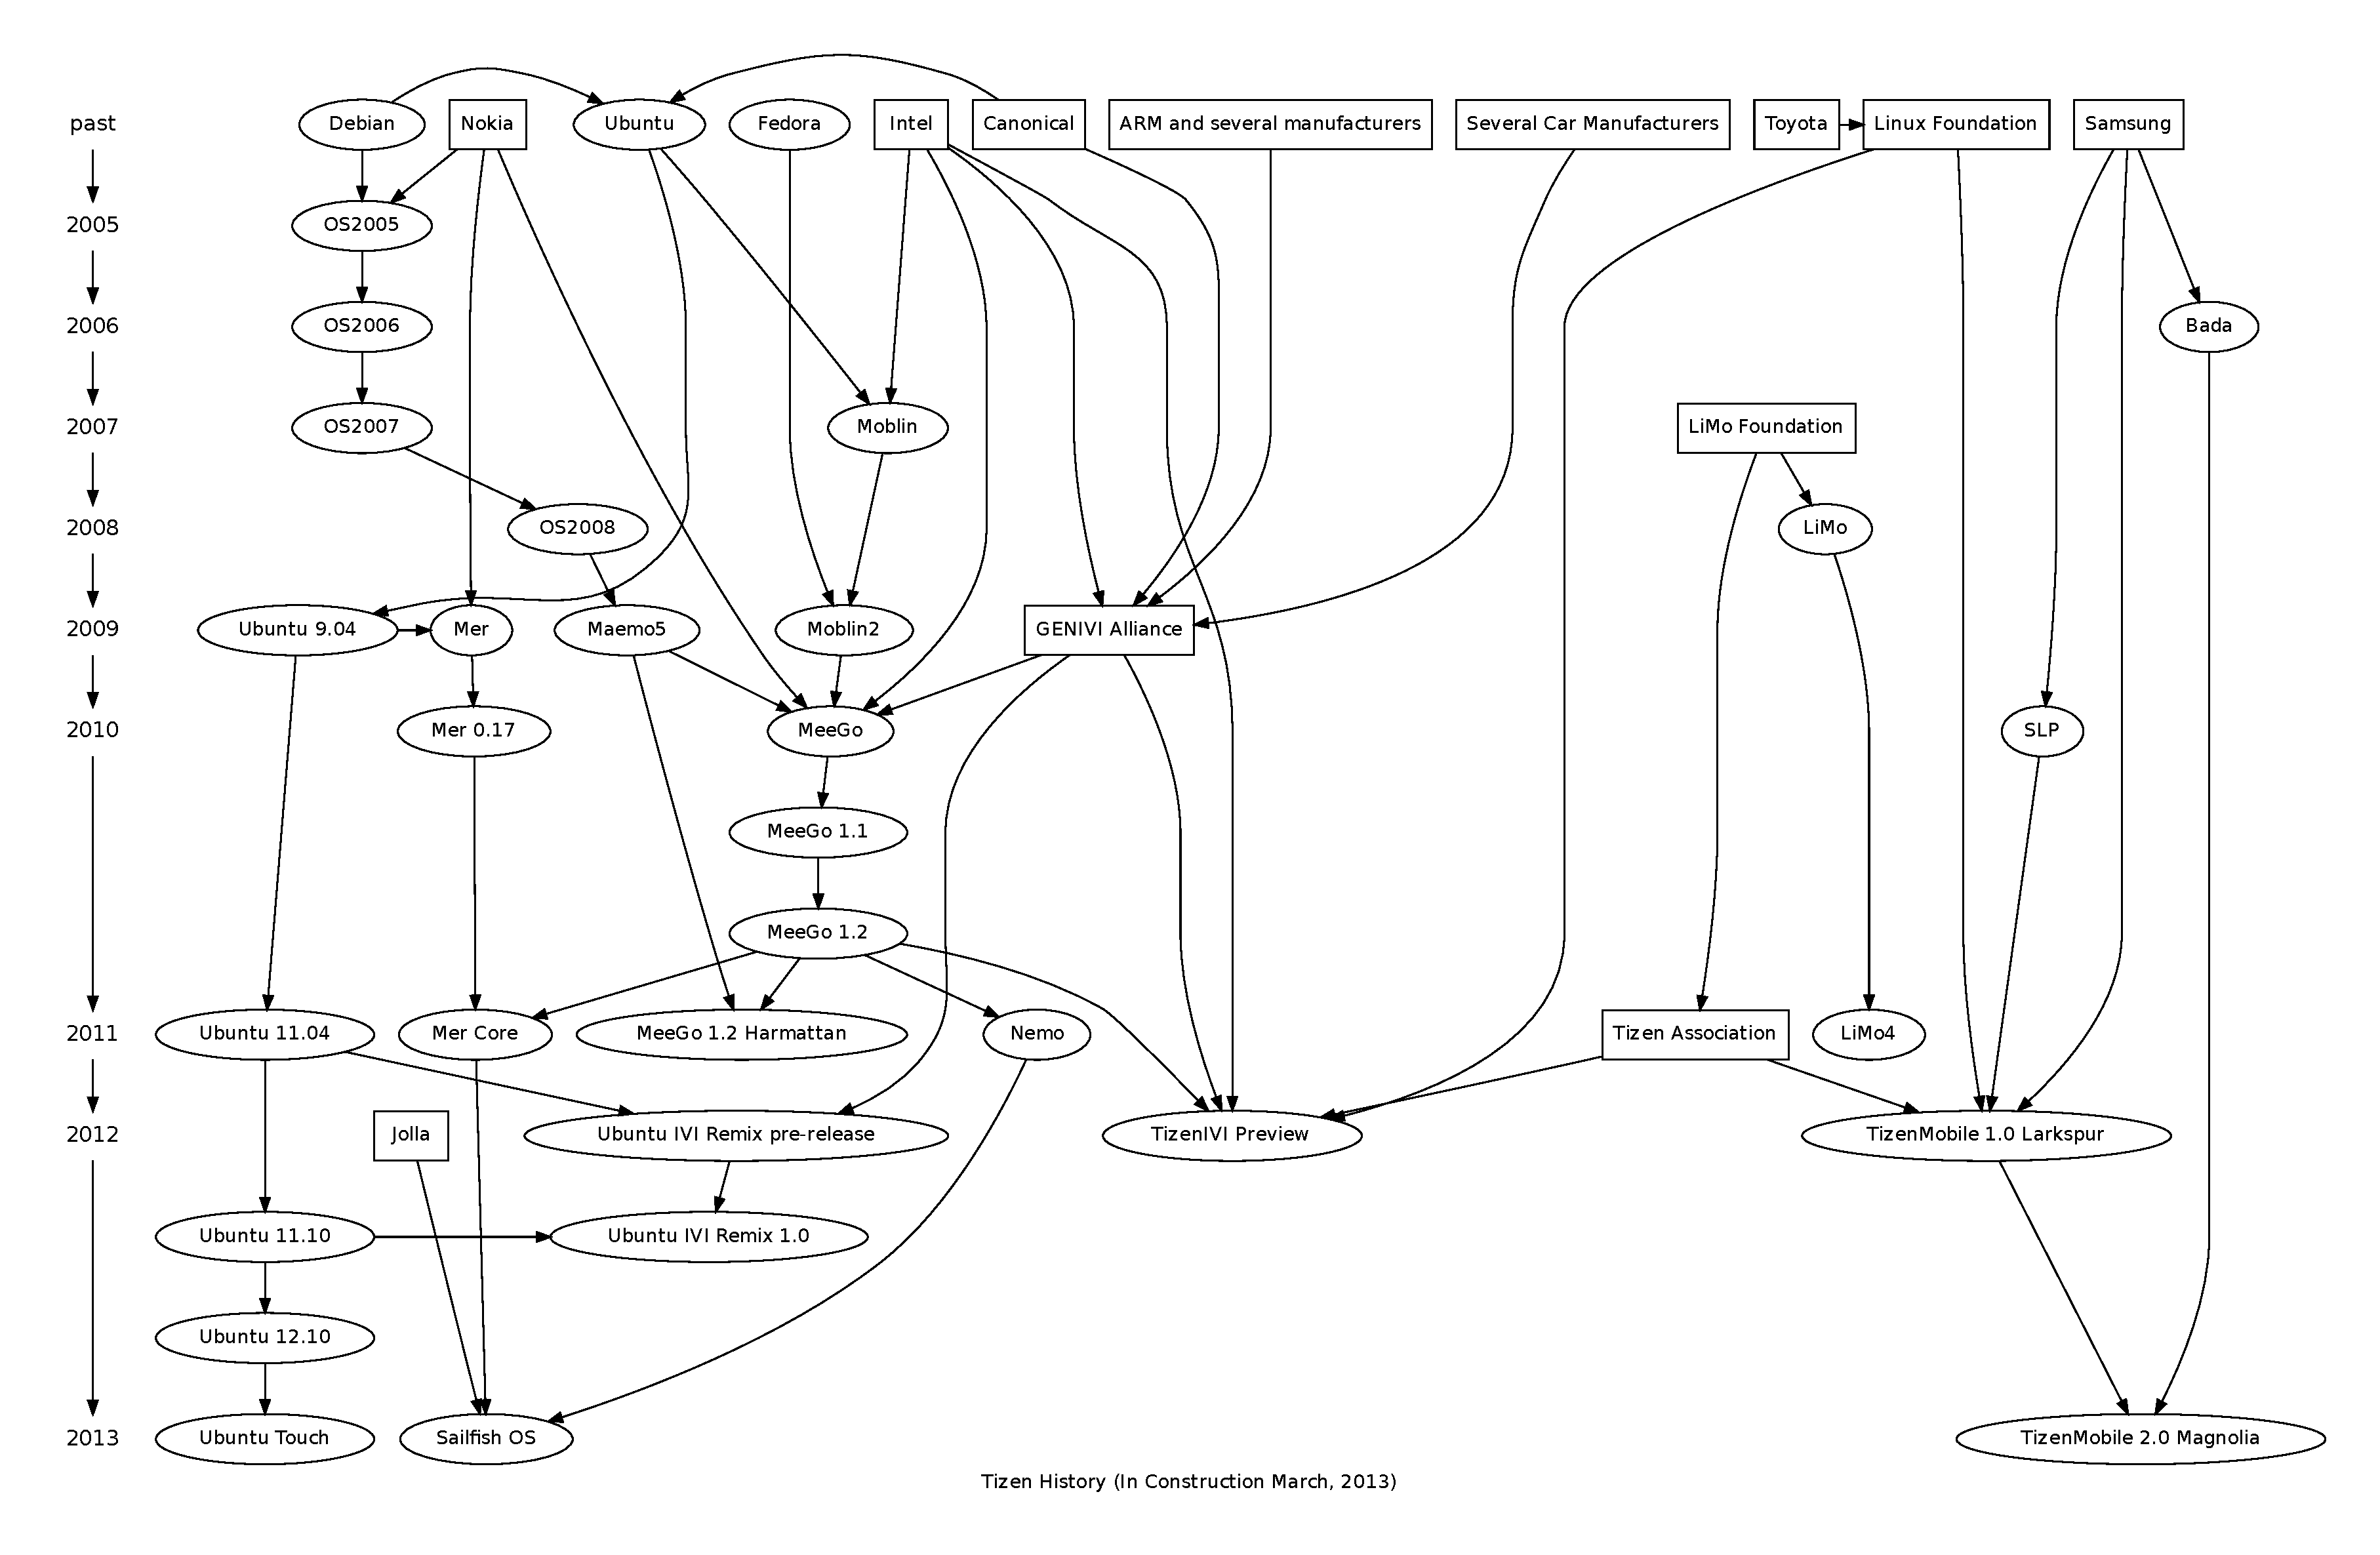
\includegraphics[height=.75\paperheight]{tizen-history}}
\end{tikzpicture}
\end{center}
\end{frame}

\begin{frame}[label=sec-2-3]{Samsung Linux Platform (SLP)}
\begin{itemize}
\item System operacyjny firmy Samsung oparty na GNU/Linuksie

\item SLP zaczynał jako system wbudowany
\end{itemize}

\note{Systemy wbudowane są inne.

Zaczynając projekt firma nie miała dużego doświadczenia z
Linuksem.  Budowała małe, wbudowane systemy (bez jednostki
zarządzania pamięcią - MMU).


\begin{itemize}
\item COMMENT Samsung = firma produkująca sprzęt i systemy wbudowane (Bada)
\end{itemize}}
\end{frame}

\begin{frame}[label=sec-2-4]{System wbudowany}
Cechy systemu wbudowanego:

\begin{itemize}
\item Realizuje jedną dobrze zdefiniowaną funkcję
\item <2-> (Typowo) Preinstalowany
\item <2-> Bardzo mocno związany z produktem
\item <3-> Produkt związany z datą wydania
\end{itemize}

\note{Oprogramowanie integralną częścią produktu.

Reżim czasowy - quick fix and dirty hack}
\end{frame}

\begin{frame}[label=sec-2-5]{System wbudowany (konsekwencje)}
\begin{itemize}
\item "Optymalizowany" pod konkretny sprzęt

\item <2-> Kontrola dostępu nie zawsze traktowana z~należytą
uwagą (/dev/exynos-mem)

\item <3-> System bardzo okrojony

\item <4-> Mnogość rozwiązań tymczasowych
\end{itemize}

\note{\begin{itemize}
\item Pliki binarne w repo - nie działa w przypadku wprowadzenia nowego
sprzętu

\item Jaki sens ma kontrola dostępu w systemie bez MMU?
\end{itemize}

Powyższe problemy wynikają z:

\begin{itemize}
\item reżimu czasowego

\item kiepskich/niewygodnych narzędzi wsparcia (kompilacji)

\item braku systemowych rozwiązań (init system który dostarcza
wymagane funkcjonalności zamiast tylko być)
\end{itemize}}
\end{frame}


\begin{frame}[label=sec-2-6]{SLP(2) circa 2010}
\begin{itemize}
\item scratchbox(1) do kompilacji skrośnej
\item init(8) z busyboksa
\item Procesy działają z uprawnieniami roota
\item Pakiety .deb do dystrybucji oprogramowania
\item <2-> Oryginalnie "projektowany" typu smartphone
\end{itemize}

\note{Wszystko z powyższego zmieniło się z czasem, bo zmieniły się aspiracje.}
\end{frame}




\begin{frame}[label=sec-2-7]{Aspiracje (potencjalne zastosowania) SLP}
\begin{itemize}
\item System operacyjny dedykowany na specjalizowane systemy:
\begin{itemize}
\item Telefony
\item Tablety
\item TV
\item Aparaty fotograficzne
\item Systemy informacyjno-rozrywkowe ("infotainment")
\item \ldots{}
\end{itemize}
\pause

\item Uniwersalny, otwarty system operacyjny na specjalizowane
urządzenia dla produktów firmy Samsung (i innych, wedle uznania)
\end{itemize}

\note{Znamy problemy, znamy aspiracje, możemy więc zacząć naprawiać
problem po problemie.}
\end{frame}

\section{Problem 1: Budowa oprogramowania}
\label{sec-3}

\begin{frame}[label=sec-3-1]{Wykorzystywane: scratchbox(1)}
scratchbox - niejawna kompilacja skrośna przez połączenie dwóch systemów:

\begin{itemize}
\item System docelowy dostarcza bibliotek
\item Narzędzia dostarczają kompilator, linker
\item chroot(8) + bind mounty + symlinki + (magia) = "spójny system"
\end{itemize}

\pause
Wady:
\begin{itemize}
\item Bardzo czasochłonny w utrzymaniu

\item Instalacja globalna /scratchbox

\item Środowisko programisty inne niż budowania

\item 1 użytkownik = 1 środowisko budowania
\end{itemize}


\note{\begin{itemize}
\item Narzędzia nie są w pełni funkcjonalnym systemem - trudna
aktualizacja

\item Środowisko programisty zupełnie inne niż budowania

\item Instalacja globalna (/scratchbox) - wymaga praw administratora

\item 1 użytkownik = 1 środowisko budowania
\end{itemize}




\begin{itemize}
\item Iluzja - tzw. niejawna cross-kompilacja

\item System co najwyżej dostateczny. Nieoptymalny.
\end{itemize}}
\end{frame}
\begin{frame}[label=sec-3-2]{Pożądane cechy środowiska budowania}
\begin{itemize}
\item Kompilacja skrośna istniejących projektów~GNU

\item Środowisko przeźroczyste dla programistów

\item Powtarzalne wyniki budowania

\item <2-> 1 użytkownik = n projektów = n środowisk

\item <2-> Środowisko nie wymagające praw administratora
\end{itemize}

\note{\begin{itemize}
\item Budujemy dystrybucję GNU/Linuksa - potrzebujemy systemu do
budowania pakietów FLOSS.

\item Powtarzalne wyniki - tak jak pbuilder w debianie.

\item Wygodne - przeźroczyste.

\item Wygodna kompilacja skrośna istniejących projektów GNU/Linux (x86
-> ARM, amd64 -> x86)

\item Środowisko przeźroczyste dla programistów i~wygodne w utrzymaniu

\item Powtarzalne wyniki budowania (niezależne od środowiska
programisty)

\item <2-> Niezależne środowiska dla różnych projektów, architektur sprzętowych, \ldots{}

\item <2-> W pełni funcjonalny system nie wymagający praw administratora
\end{itemize}}
\end{frame}

\begin{frame}[label=sec-3-3]{Alternatywy}
\begin{itemize}
\item Natywna kompilacja

\item Android - "make world"

\item Debian/Ubuntu - multiarch

\item Maemo/MeeGo - scratchbox 2
\end{itemize}

\note{\begin{itemize}
\item Natywna kompilacja - niemożliwa z przyczyn technicznych - brak
sprzętu lub codziennie inny sprzęt

\item Android - "make world" - nie przystaje do kompilacji projektów GNU/Linuksa

\item Debian/Ubuntu - multiarch - pieśń przyszłości

\item Maemo/MeeGo - scratchbox2 - elastyczny i skompilikowany
\end{itemize}


NIEOPISANE: - emulacja wszysktkiego za pomocą qemu - niemożliwe z
przyczyn technicznych (kompilacja webkitta)}
\end{frame}

\begin{frame}[label=sec-3-4]{scratchbox 2 + samsung}
scratchbox 2:
\begin{itemize}
\item Biblioteka zmieniająca odwzorowanie ścieżek przy próbie dostępu
(LD PRELOAD)
\item Reguły w języku Lua
\item Nie wymaga praw administratora
\item Skomplikowana konfiguracja
\end{itemize}

\pause\vskip0.5cm

sbs - SLP/Samsung Build System
\begin{itemize}
\item Skrypt do stworzenia kompletnego środowiska (debootstrap + sb2-init + sb2)
\item Reguły specyficzne dla SLP
\end{itemize}
\end{frame}

\begin{frame}[label=sec-3-5]{scratchbox 2 + sbs (przykład)}
\begin{center}
\includegraphics<1>[width=\textwidth]{images/sb2-m1}
\includegraphics<2>[width=\textwidth]{images/sb2-0}
\includegraphics<3>[width=\textwidth]{images/sb2-1}
\includegraphics<4>[width=\textwidth]{images/sb2-2}
\includegraphics<5>[width=\textwidth]{images/sb2-3}
\end{center}
\end{frame}

\begin{frame}[label=sec-3-6]{System budowania dziś}
\begin{itemize}
\item openSUSE build service (OBS) - adresuje problemy, których nie
rozwiązywał sbs
\begin{itemize}
\item Zaprojektowany z myślą o wymaganiach grupy SCM
\item Nastawiony na zarządzanie dużą ilością projektów
\item Scentralizowany i łatwo zarządzalny (web ui)
\end{itemize}

\item <2-> Gerrit do oceny jakości kodu
\end{itemize}

\note{\begin{itemize}
\item Instaluje system docelowy (armel), binarki odpalane przez qemu,
nieliczne - dostarczone prekompilowane pakiety natywne i własny
menedżer pakietów do instalacji pakietów z różnych architektur

\item chroot(8), system docelowy + qemu-static-ARCH, zmodyfikowane
pakiety i menedżer pakietów (instalacja z różnych architektur)
\end{itemize}

Wygodny dla SCMu, dla programistów - średnio.}
\end{frame}

\section{Problem 2: init(8)}
\label{sec-4}

\begin{frame}[label=sec-4-1]{Stan zastany}
\begin{itemize}
\item init(8) z busyboksa
\item /etc/rc.d/rc.sysinit
\item Skrypty serwisów - od 1 linii  ("foo \&") do 1xxx

\item Synchronizacja uruchamiania usług:

while [ -e /tmp/foo ]; do sleep 1; done \&\& bar \&

\item <2-> System "zoptymalizowany" - czasem działał
\end{itemize}

\note{\begin{itemize}
\item init(8) z busyboksa - co najmniej ograniczony - nie wspiera
\end{itemize}
koncepcji runleveli (a takowe były wykorzystywane przy starcie
SLP, zrobione ręcznie).}
\end{frame}
\begin{frame}[label=sec-4-2]{\# ps -ef (składowe systemu)}
\begin{itemize}
\item Pojedyncze programy realizujące interfejs użytkownika (GUI)

\item <2-> Bardzo dużo usług klient/serwer (demonów) korzystających z
różnorakich mechanizmów IPC:
\begin{itemize}
\item Gniazda UNIX
\item D-Bus
\item SYSV IPC
\item vconf (pliki + inotify(2))
\end{itemize}

\item <3-> Serwisy restartujące krytyczne usługi i aplikacje:
\begin{itemize}
\item menu-daemon -> menu-screen
\end{itemize}
\end{itemize}
\end{frame}

\begin{frame}[label=sec-4-3]{Alternatywne rozwiązania}
\begin{itemize}
\item sysvinit+insserv (tagi LSB)
\item upstart
\item systemd (v25)
\begin{itemize}
\item <2-> Deklaratywny opis systemu
\item <2-> Uruchamianie usług na żądanie (socket activation)
\item <2-> Uproszczenie zależności usług (dzięki powyższemu)
\item <2-> Domyślne zrównoleglanie uruchamianych usług
\item <2-> systemd --user
\end{itemize}
\end{itemize}

\note{\begin{itemize}
\item sysvinit - kosztowny i niewiele wnosi (skrypty i tak muszą być
przepisane)

\item upstart - bazuje na eventach, wymaga wyspecyfikowania wszystkich
zależności usługi. Niezarządzalne.

\item systemd
\end{itemize}}
\end{frame}
\begin{frame}[label=sec-4-4]{Wdrożenie systemd}
Konsekwencje wdrożenia systemd:

\pause

\begin{itemize}
\item Brak zmian
\end{itemize}

\pause

Analiza działania systemu za pomocą narzędzi:
\begin{itemize}
\item strace
\item systemd-analyze
\item bootgraph.pl (kernel)
\item (systemd-)bootchart
\end{itemize}

\pause
Symptomy problemów:
\begin{itemize}
\item Niewykorzystane I/O, CPU
\item Usługi uruchamiane sekwencyjnie
\end{itemize}


\note{System działał, ale na pewno nie uruchamiał się szybciej (na co
liczyliśmy). Czasem działał wolniej.

\begin{itemize}
\item <3-> Usługi uruchamiane sekwencyjnie - co oznacznie niepoprawnie
opisane zależności.

\item Jak ustalić poprawną kolejność?
\end{itemize}}
\end{frame}
\begin{frame}[label=sec-4-5]{Zbieranie dokładnych informacji - auditd}
\begin{itemize}
\item Podsystem audytu w Linuksie pozwala na bardzo dokładne śledzenie
zachowania systemu.

\item <2-> IPC oznacza konieczność synchronizacji uruchamiania usług:
\begin{itemize}
\item Dostęp do plików/konfiguracji - open(2), write(2), inotify(2)
\item Usługi klient/serwer - connect(2), bind(2)
\end{itemize}

\item <3-> Automatyczne generowanie grafów zależności (aureport +
perl + graphwiz/dot)
\end{itemize}

\note{Określenie Wywołań systemowych oznaczających synchronizaję (IPC)
\begin{itemize}
\item open(2), write(2), inotify(2) -
\item connect(2), bind(2)
\end{itemize}}
\end{frame}
\begin{frame}[label=sec-4-6]{auditd + dot (przykład)}
\begin{center}
\includegraphics<1>[width=\textwidth]{images/auditd-0}
\includegraphics<2>[width=\textwidth]{images/auditd-1}
\includegraphics<3>[width=\textwidth]{images/auditd-2}
\includegraphics<4>[width=\textwidth]{images/auditd-3}
\includegraphics<5>[width=\textwidth]{images/auditd-4}
\includegraphics<6>[width=\textwidth]{images/auditd-5}
\includegraphics<7>[width=\textwidth]{images/auditd-6}
\includegraphics<8>[width=\textwidth]{images/auditd-7}
\includegraphics<9>[width=\textwidth]{images/auditd-8}
\end{center}
\end{frame}
\begin{frame}[label=sec-4-7]{auditd - uniwersalne narzędzie}
Możliwe śledzenie wywołań systemowych:
\begin{itemize}
\item sync(2), f*sync(2)
\item execve(3)
\item \ldots{}
\end{itemize}
\end{frame}

\begin{frame}[label=sec-4-8]{init(8) dziś i jutro}
\begin{itemize}
\item systemd v204 + natywna konfiguracja

\item Wiele serwisów uruchamianych na żądanie, wiele rozważanych (Xorg)
\end{itemize}


\note{fdatasync(2) w zniszczył wydajność Firefoxa 3 (awesomebar), ale
nie tylko tam.}
\end{frame}

\section{Problem 3: Niezawodność systemu}
\label{sec-5}

\begin{frame}[label=sec-5-1]{Stan zastany}
\begin{itemize}
\item Większość programów działa z prawami administratora (w tym
window manager)

\item Zatrzymanie procesu często kończy się wymuszonym restarem
systemu (watchdog)
\end{itemize}

\pause
W konsekwencji:
\begin{itemize}
\item Niemożliwe do zrealizowania jakiekolwiek security
\end{itemize}

\pause
Systemy Uniksowe dostarczyły podstawowego rozwiązania zagadnienia
security ponad 40 lat temu - użytkownicy, grupy (tzw. DAC).
\end{frame}

\begin{frame}[label=sec-5-2]{Zarządzanie sesją użytkownika}
\begin{itemize}
\item Programy sesji użytkownika mają podobne wymagania jak systemowe:
\begin{itemize}
\item Zarządzanie cyklem życia (w tym automatyczny restart)
\item Uruchamianie usług na żądanie
\item Monitorowanie
\end{itemize}

\item <2-> systemd --user
\begin{itemize}
\item Sesja graficzna (xorg-launch-helper)
\item Sesyjny D-Bus uruchamiany na żądanie
\end{itemize}
\end{itemize}
\end{frame}

\begin{frame}[label=sec-5-3]{Niezawodność dziś i jutro}
\begin{itemize}
\item Usługi nieuprzywilejowane w osobnej sesji

\item SMACK do drobnoziarnistej kontroli dostępu
\end{itemize}
\end{frame}
\section{Dalsze kroki}
\label{sec-6}

\begin{frame}[label=sec-6-1]{Quo vadis TizenOS?}
\begin{itemize}
\item Więcej GNU/Linuksa w Tizenie
\item <2-> Więcej Tizena w GNU/Linuksie
\end{itemize}
\end{frame}

\section{Q\&A}
\label{sec-7}

\begin{frame}[label=sec-7-1]{Pytania i odpowiedzi}
Autor niniejszej prezentacji nie posiada informacji czy i~kiedy będzie
wydany wykorzystujący Tizena:

\begin{itemize}
\item telefon
\item telewizor
\item samochód
\item czołg(?)
\end{itemize}

:)
\end{frame}

\begin{frame}[label=sec-7-2]{Dziękuję za uwagę}
Karol Lewandowski <k.lewandowsk@samsung.com>

lmctl @freenode (\#tizen)
\end{frame}

\begin{frame}[label=sec-7-3]{Linki}
\begin{itemize}
\item sbs (wartość historyczna): \url{https://review.tizen.org/git/?p=tools/sbs.git;a=summary}

\item Gerrit:  \url{http://review.tizen.org/gerrit}

\item Lista tizen-dev: \url{https://lists.tizen.org/pipermail/dev/}

\item Grafy auditd: \url{https://wiki.tizen.org/wiki/System/Dependency_graphs}

\item xorg-launch-helper: \url{https://github.com/sofar/xorg-launch-helper}

\item systemd --user units: \url{https://github.com/sofar/user-session-units}
\end{itemize}
\end{frame}
% Emacs 23.3.1 (Org mode 8.0.7)
\end{document}
